\documentclass{beamer}

\title{\textbf{Digi}Approval}
\author{Daniel Axtens, Andrew Donnellan, Benjamin Roberts}

\begin{document}

\maketitle

\begin{frame}
  \frametitle{Summary}
  \begin{itemize}
  \item Challenge: simple, online system to get all the necessary approvals to run events.
  \item Our solution: Online workflow based system
    \begin{itemize}
    \item Centralised: all contact and information in one place
    \item Continuity: deal with one ``account manager'' throughout process.
    \end{itemize}
  \end{itemize}
\end{frame}


\begin{frame}
\frametitle{Workflow}
\begin{figure}[h!]
  \centering
  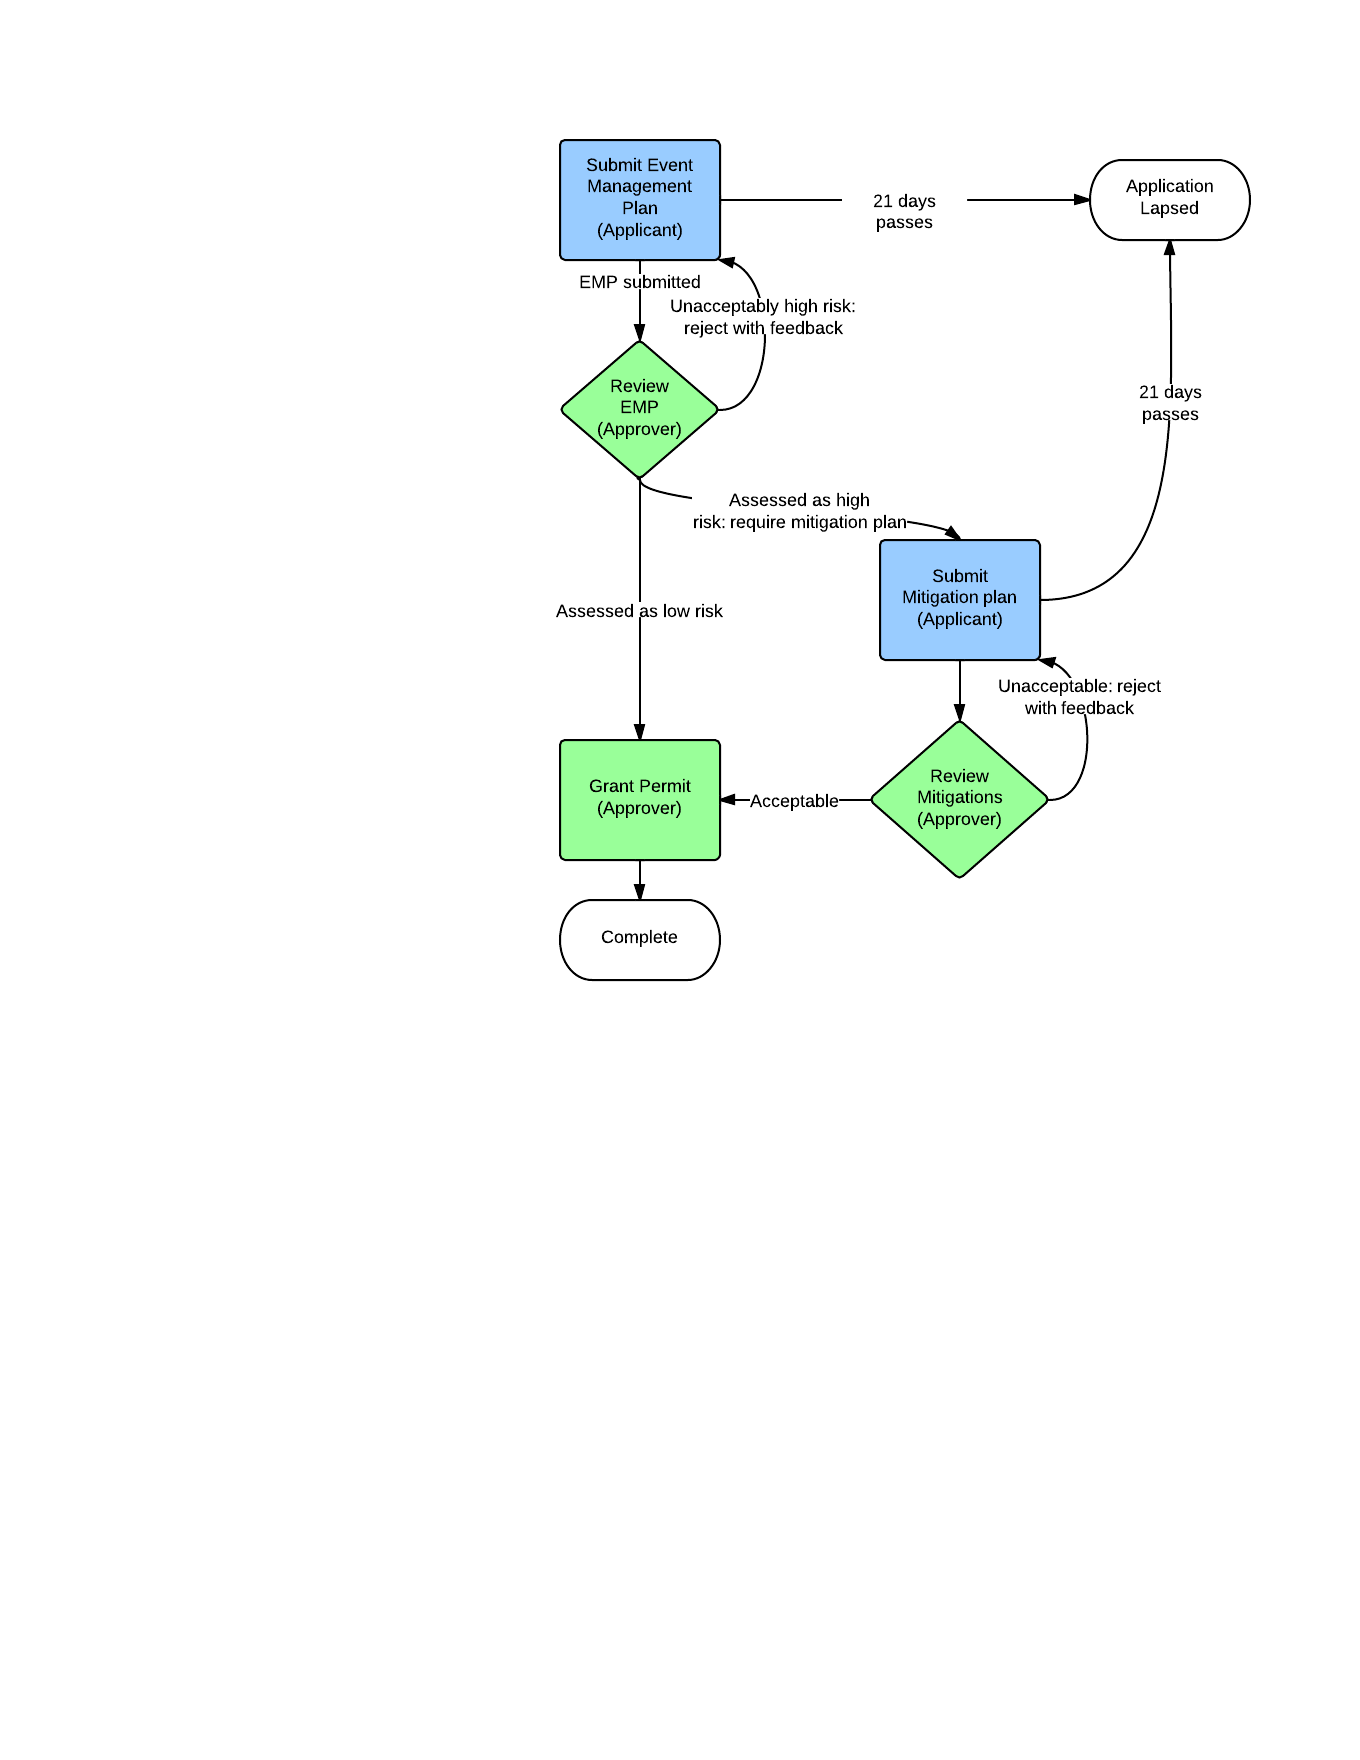
\includegraphics[scale=0.25]{./imgs/sample-workflow.png}  
\end{figure}
\end{frame}

\begin{frame}
  \frametitle{User Mockup}
  \begin{figure}[h!]
    \centering
    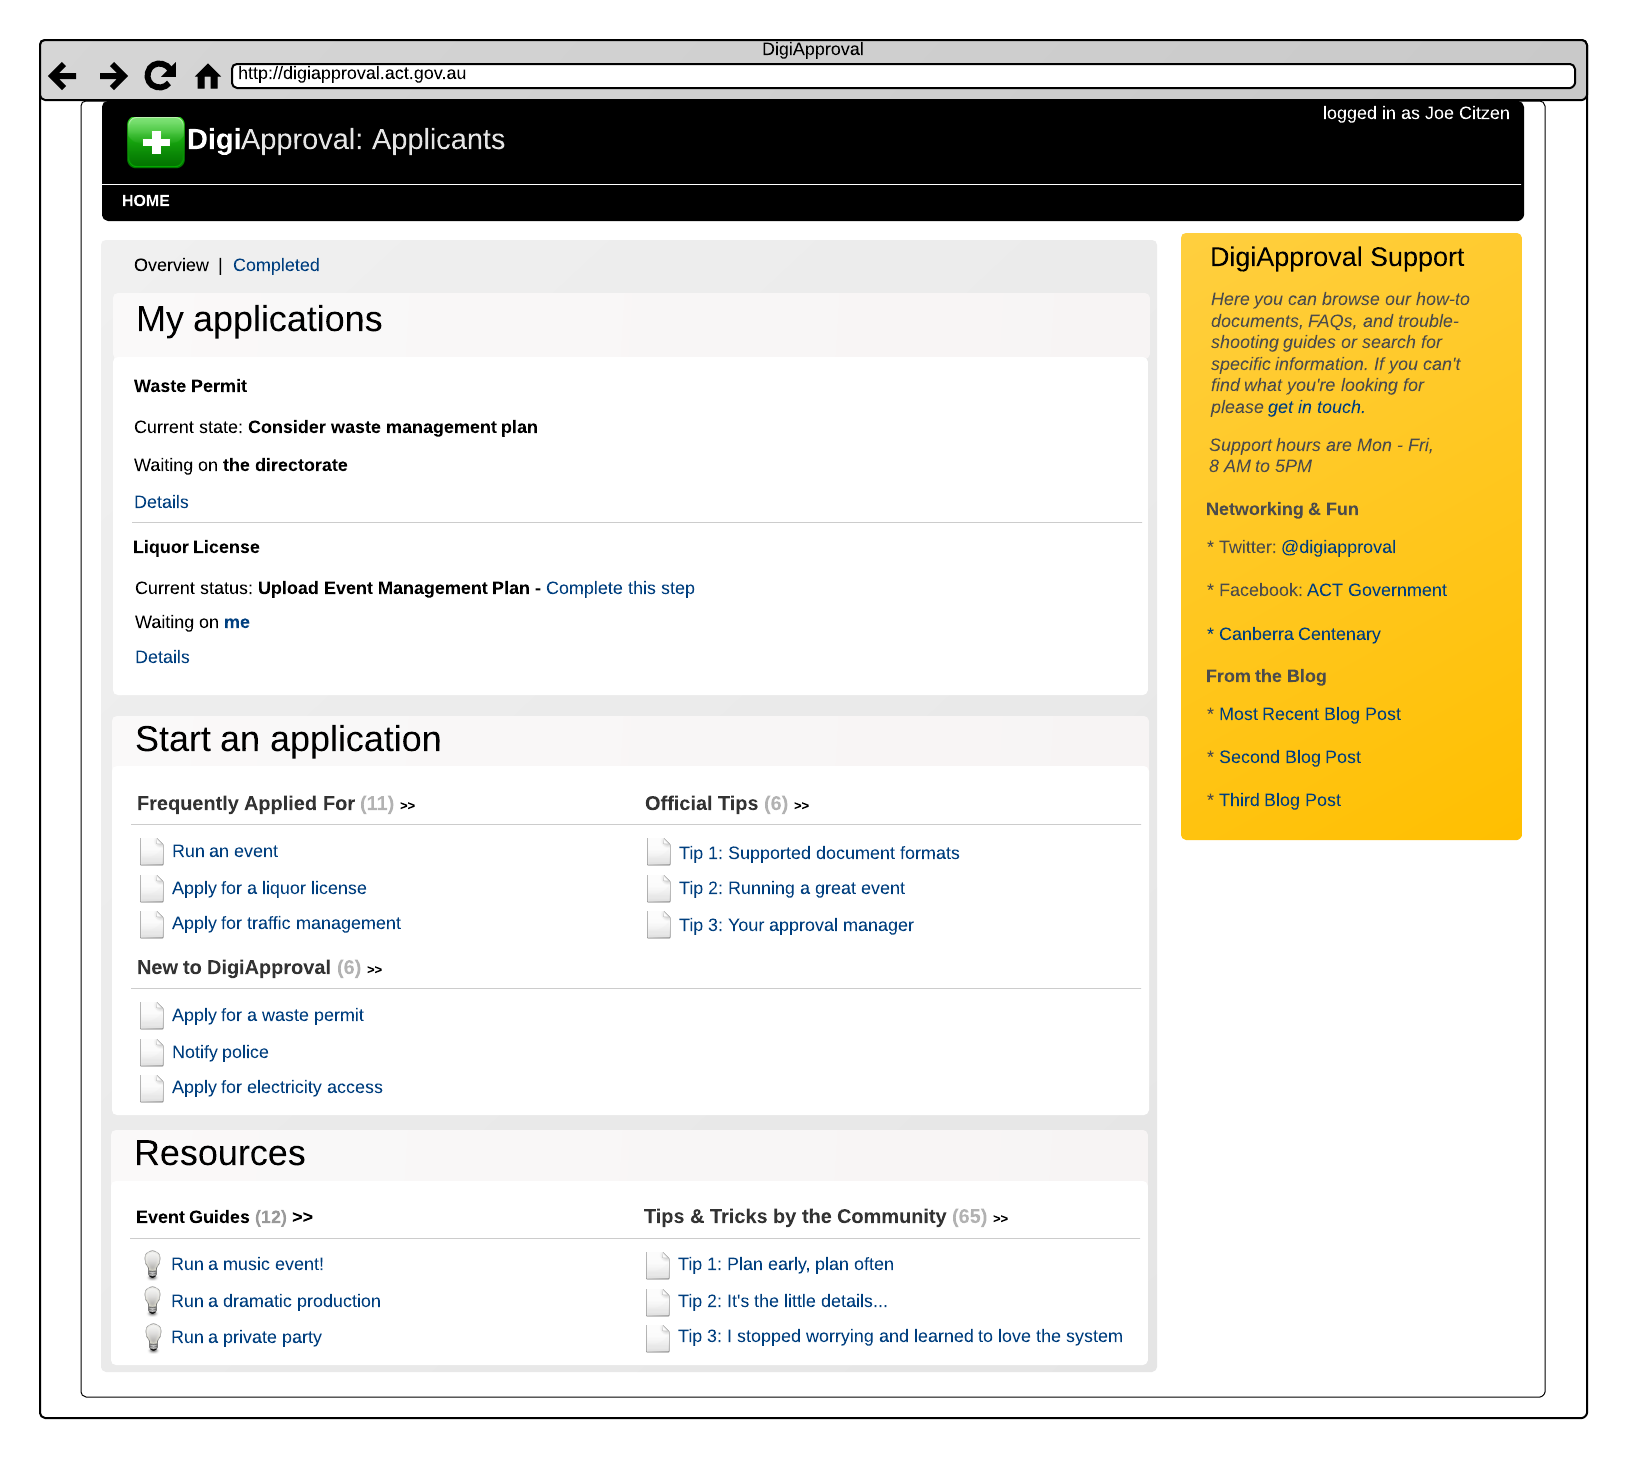
\includegraphics[width=0.8\textwidth]{./imgs/user-wireframe.png}
  \end{figure}
\end{frame}

\begin{frame}
  \frametitle{Approver/Account Manager Mockup}
  \begin{figure}[h!]
    \centering
    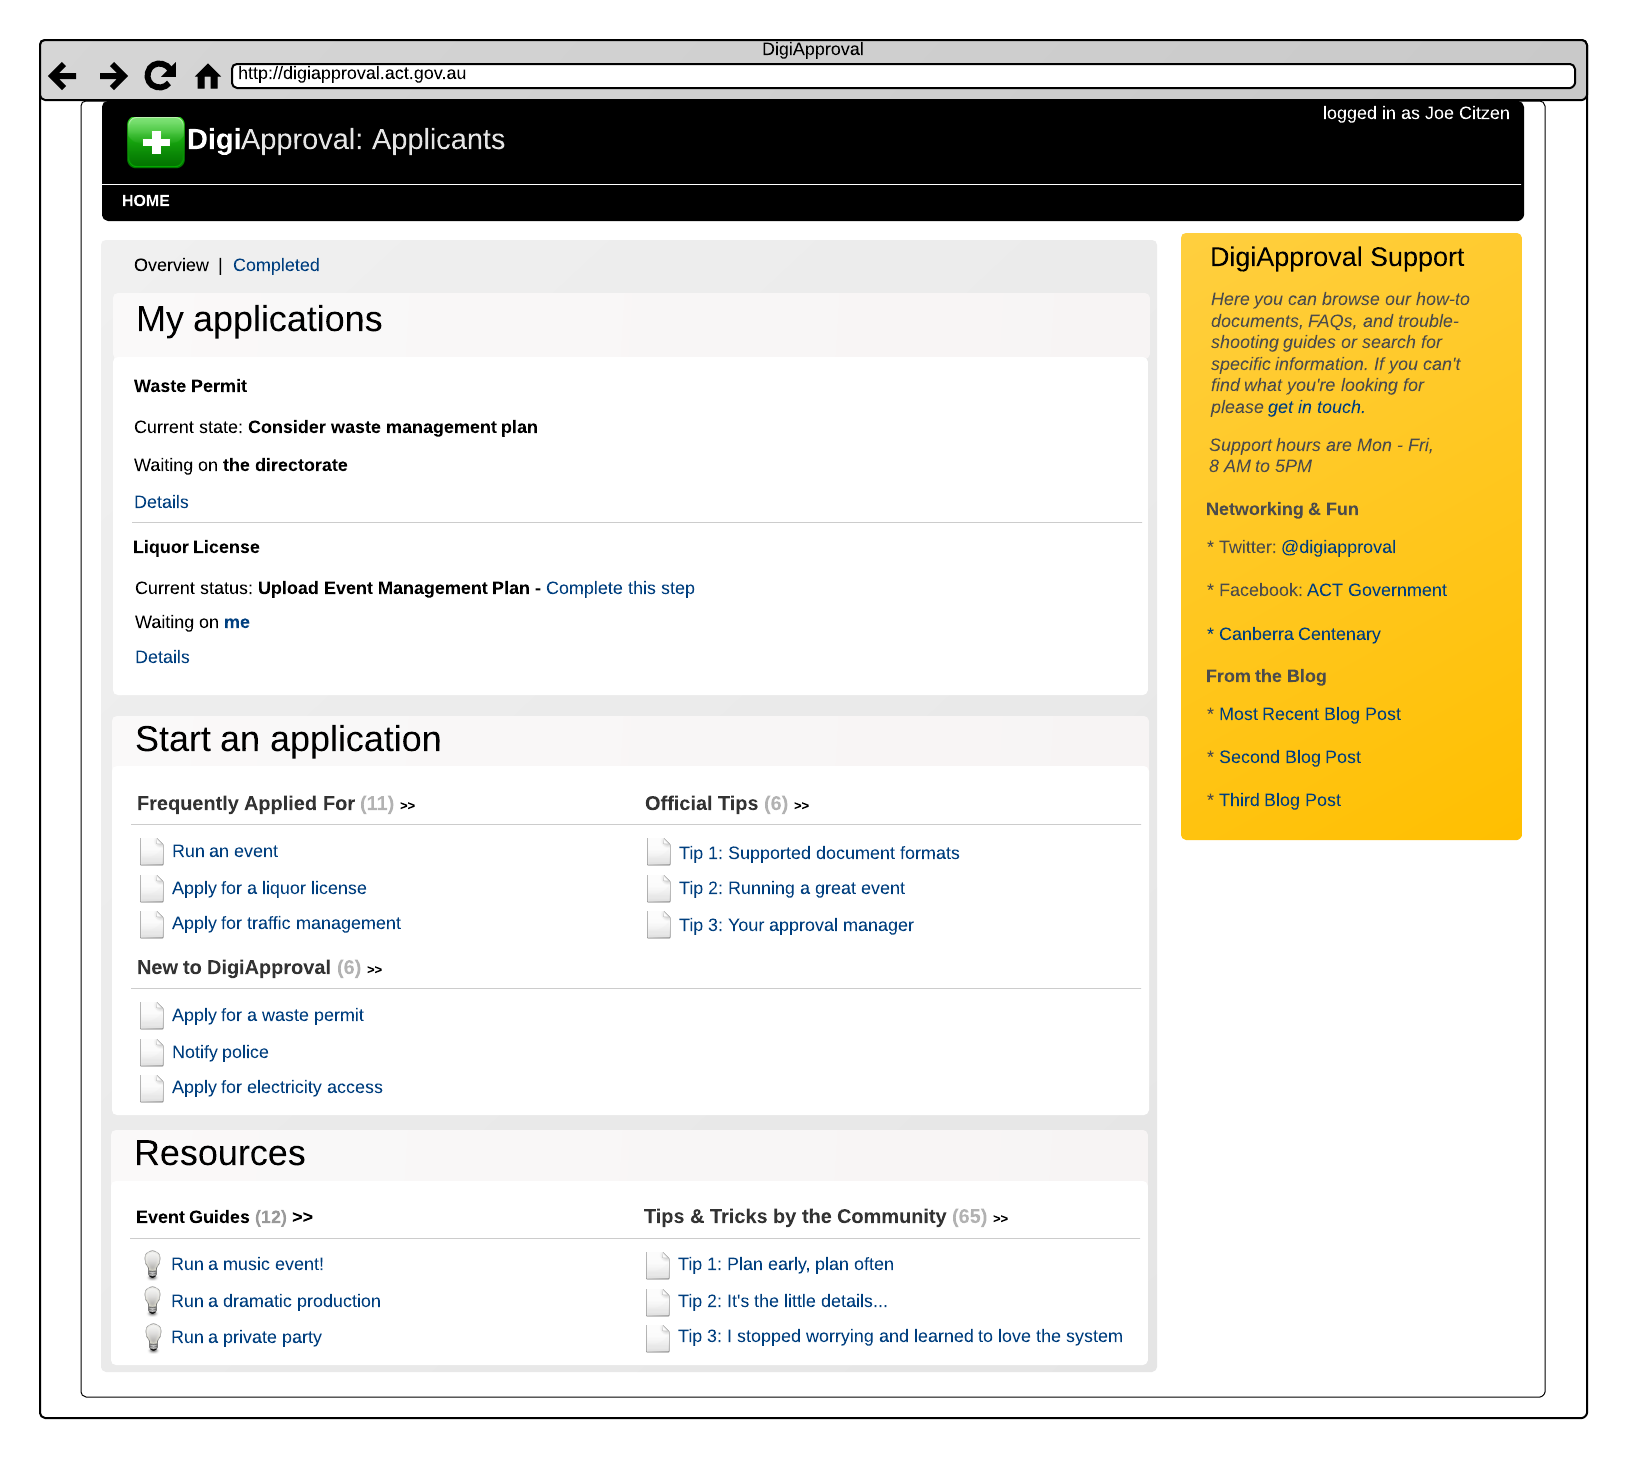
\includegraphics[width=0.8\textwidth]{./imgs/approver-wireframe.png}
  \end{figure}
\end{frame}

\begin{frame}
  \frametitle{Technology}
  \begin{figure}[h!]
    \centering
    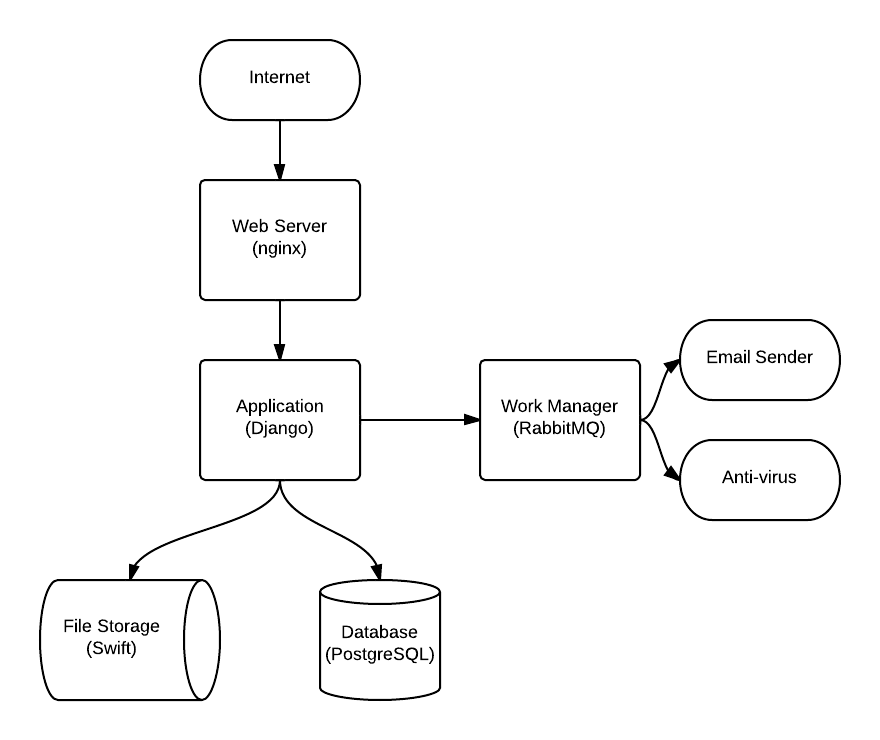
\includegraphics[width=0.8\textwidth]{./imgs/tech-overview.png}
  \end{figure}
\end{frame}

\begin{frame}
  \frametitle{Milestones}
  \begin{itemize}
  \item By the end of week 1: Infrastructure set up, technology stack
    working.
  \item By the end of week 4: Static (manually coded) workflows work.
  \item During week 9/10: Dynamic (user entered) workflows can be
    created and work.
  \item Remaining time:
    \begin{itemize}
    \item Polish the user interface.
    \item Catch up on any missed milestones.
    \item Write case study.
    \end{itemize}
  \end{itemize}
\end{frame}

\begin{frame}
  \frametitle{What we would need}
  \begin{itemize}
  \item Costs: Hosting
  \item Involvement from directorate staff: 
    \begin{itemize}
    \item Sample workflow to implement
    \item Feedback on our implementation at milestones
    \item Future: integration with ACT payment system
    \end{itemize}
  \end{itemize}
\end{frame}

\end{document}